\chapter*{What's New in v2.1}
%===========================
\addcontentsline{toc}{chapter}{What's New in v2.1}

\section*{New Science}
%---------------------
\addcontentsline{toc}{section}{New Science}

\begin{description}
\item[Updated microwave sea surface emissivity model] The FASTEM4/5 microwave sea surface emissivity models have been implemented. FASTEM5 is the default (via a file loaded during initialisation) and FASTEM4 \citep{QLiu_2011} can be selected by specifying the appropriate data file during CRTM initialisation. The previous model, a combination of FASTEM1 \citep{Fastem1} and a low frequency model \citep{Kazumori_2008}, can still be invoked via the options input to the CRTM functions. An indication of the differences between the FASTEM5/4/1 microwave sea surface emissivity models for some AMSU-A channels (NOAA-15 through MetOp-A) are shown in figures \ref{fig:fastem_impact_amsua_ch1} to \ref{fig:fastem_impact_amsua_ch15}.


\item[Updated microwave land surface emissivity model] The microwave land emissivity model now uses more information about the surface characteristics, specifically soil and vegetation types as well as the leaf area index (LAI), to compute the emissivity. An indication of the impact of the updated microwave land surface emissivity model for some NOAA-18 AMSU-A channels is shown in figure \ref{fig:mw_land_impact_amsua_ch1}.

 
\item[Non-LTE for hyperspectral infrared sensors] A model to correct daytime radiances for the non-LTE effect in the shortwave infrared channels has been implemented \citep{Chen_2012}. Currently the correction is applied only to the hyperspectral infrared sensors; AIRS (Aqua), IASI (MetOp-A/B), and CrIS (Suomi NPP). An indication of the impact of including the non-LTE correction for some affected MetOp-A IASI channels is shown in figure \ref{fig:nlte_impact_iasi_metop-a}.


\item[Successive Order of Interaction (SOI) radiative transfer algorithm] An alternative radiative transfer (RT) solution algorithm \citep{SOI_1} has been implemented and can be selected for use via the options input to the CRTM functions. The default RT solver still remains the Advanced Doubling-Adding (ADA) algorithm \citep{Liu_2006}\footnote{The ADA implementation in the CRTM uses the Matrix Operator Method (MOM) \citep{Liu_1996} for calculating layer quantities}.

\end{description}

\begin{figure}[H]
  \centering
  \includegraphics[scale=0.4]{graphics/New/FASTEM/amsua-ch1.eps}
  \caption[Effect of FASTEM changes in AMSU-A channel 1]{GSI single-cycle run (2012060700) results for AMSU-A channel 1 (with QC) comparing use of FASTEM5 (top panels), FASTEM4 (middle pannels), and FASTEM1 (bottom panels). The data plots are, from left to right, simple scatterplot, simple histogram, and 2-D density map (brighter colour indicates higher point density).}
  \label{fig:fastem_impact_amsua_ch1}
\end{figure}

\begin{figure}[H]
  \centering
  \includegraphics[scale=0.4]{graphics/New/FASTEM/amsua-ch2.eps}
  \caption[Effect of FASTEM changes in AMSU-A channel 2]{GSI single-cycle run (2012060700) results for AMSU-A channel 2 (with QC) comparing use of FASTEM5 (top panels), FASTEM4 (middle pannels), and FASTEM1 (bottom panels). The data plots are, from left to right, simple scatterplot, simple histogram, and 2-D density map (brighter colour indicates higher point density).}
  \label{fig:fastem_impact_amsua_ch2}
\end{figure}

\begin{figure}[H]
  \centering
  \includegraphics[scale=0.4]{graphics/New/FASTEM/amsua-ch3.eps}
  \caption[Effect of FASTEM changes in AMSU-A channel 3]{GSI single-cycle run (2012060700) results for AMSU-A channel 3 (with QC) comparing use of FASTEM5 (top panels), FASTEM4 (middle pannels), and FASTEM1 (bottom panels). The data plots are, from left to right, simple scatterplot, simple histogram, and 2-D density map (brighter colour indicates higher point density).}
  \label{fig:fastem_impact_amsua_ch3}
\end{figure}

\begin{figure}[H]
  \centering
  \includegraphics[scale=0.4]{graphics/New/FASTEM/amsua-ch15.eps}
  \caption[Effect of FASTEM changes in AMSU-A channel 15]{GSI single-cycle run (2012060700) results for AMSU-A channel 15 (with QC) comparing use of FASTEM5 (top panels), FASTEM4 (middle pannels), and FASTEM1 (bottom panels). The data plots are, from left to right, simple scatterplot, simple histogram, and 2-D density map (brighter colour indicates higher point density).}
  \label{fig:fastem_impact_amsua_ch15}
\end{figure}

\begin{figure}[htp]
  \centering
  \begin{tabular}{c c}
    \tblhd{Old MW land emissivity model (CTL)} & \tblhd{New MW land emissivity model (SEN)}\\
    \multicolumn{2}{c}{\textsf{Channel 1}}\\
    \includegraphics[bb=0   280 395 529,clip,scale=0.6]{graphics/New/MW_Land/amsua_n18-ch1_2.eps} &
    \includegraphics[bb=395 280 794 529,clip,scale=0.6]{graphics/New/MW_Land/amsua_n18-ch1_2.eps}\\
    \hline\\
    \multicolumn{2}{c}{\textsf{Channel 2}}\\
    \includegraphics[bb=0   0 395 245,clip,scale=0.6]{graphics/New/MW_Land/amsua_n18-ch1_2.eps} &
    \includegraphics[bb=395 0 794 245,clip,scale=0.6]{graphics/New/MW_Land/amsua_n18-ch1_2.eps}\\
    \hline\\
    \multicolumn{2}{c}{\textsf{Channel 3}}\\
    \includegraphics[bb=0   280 395 529,clip,scale=0.6]{graphics/New/MW_Land/amsua_n18-ch3_4.eps} &
    \includegraphics[bb=395 280 794 529,clip,scale=0.6]{graphics/New/MW_Land/amsua_n18-ch3_4.eps}
  \end{tabular}
  \caption[Effect of Microwave Land Emissivity changes in NOAA-18 AMSU-A channels 1-3]{Map of NOAA-18 AMSU-A channels 1-3 brightness temperature differences (observed-calculated) for the 2010073112 period for a GSI-GFS full cycle run from 1 July 2010 to 1 August 2010. The control run (CTL) uses the currently operational microwave land emissivity model, and the sensitivity run (SEN) uses the updated microwave land emissivity model.}
  \label{fig:mw_land_impact_amsua_ch1}
\end{figure}

\begin{figure}[H]
  \centering
  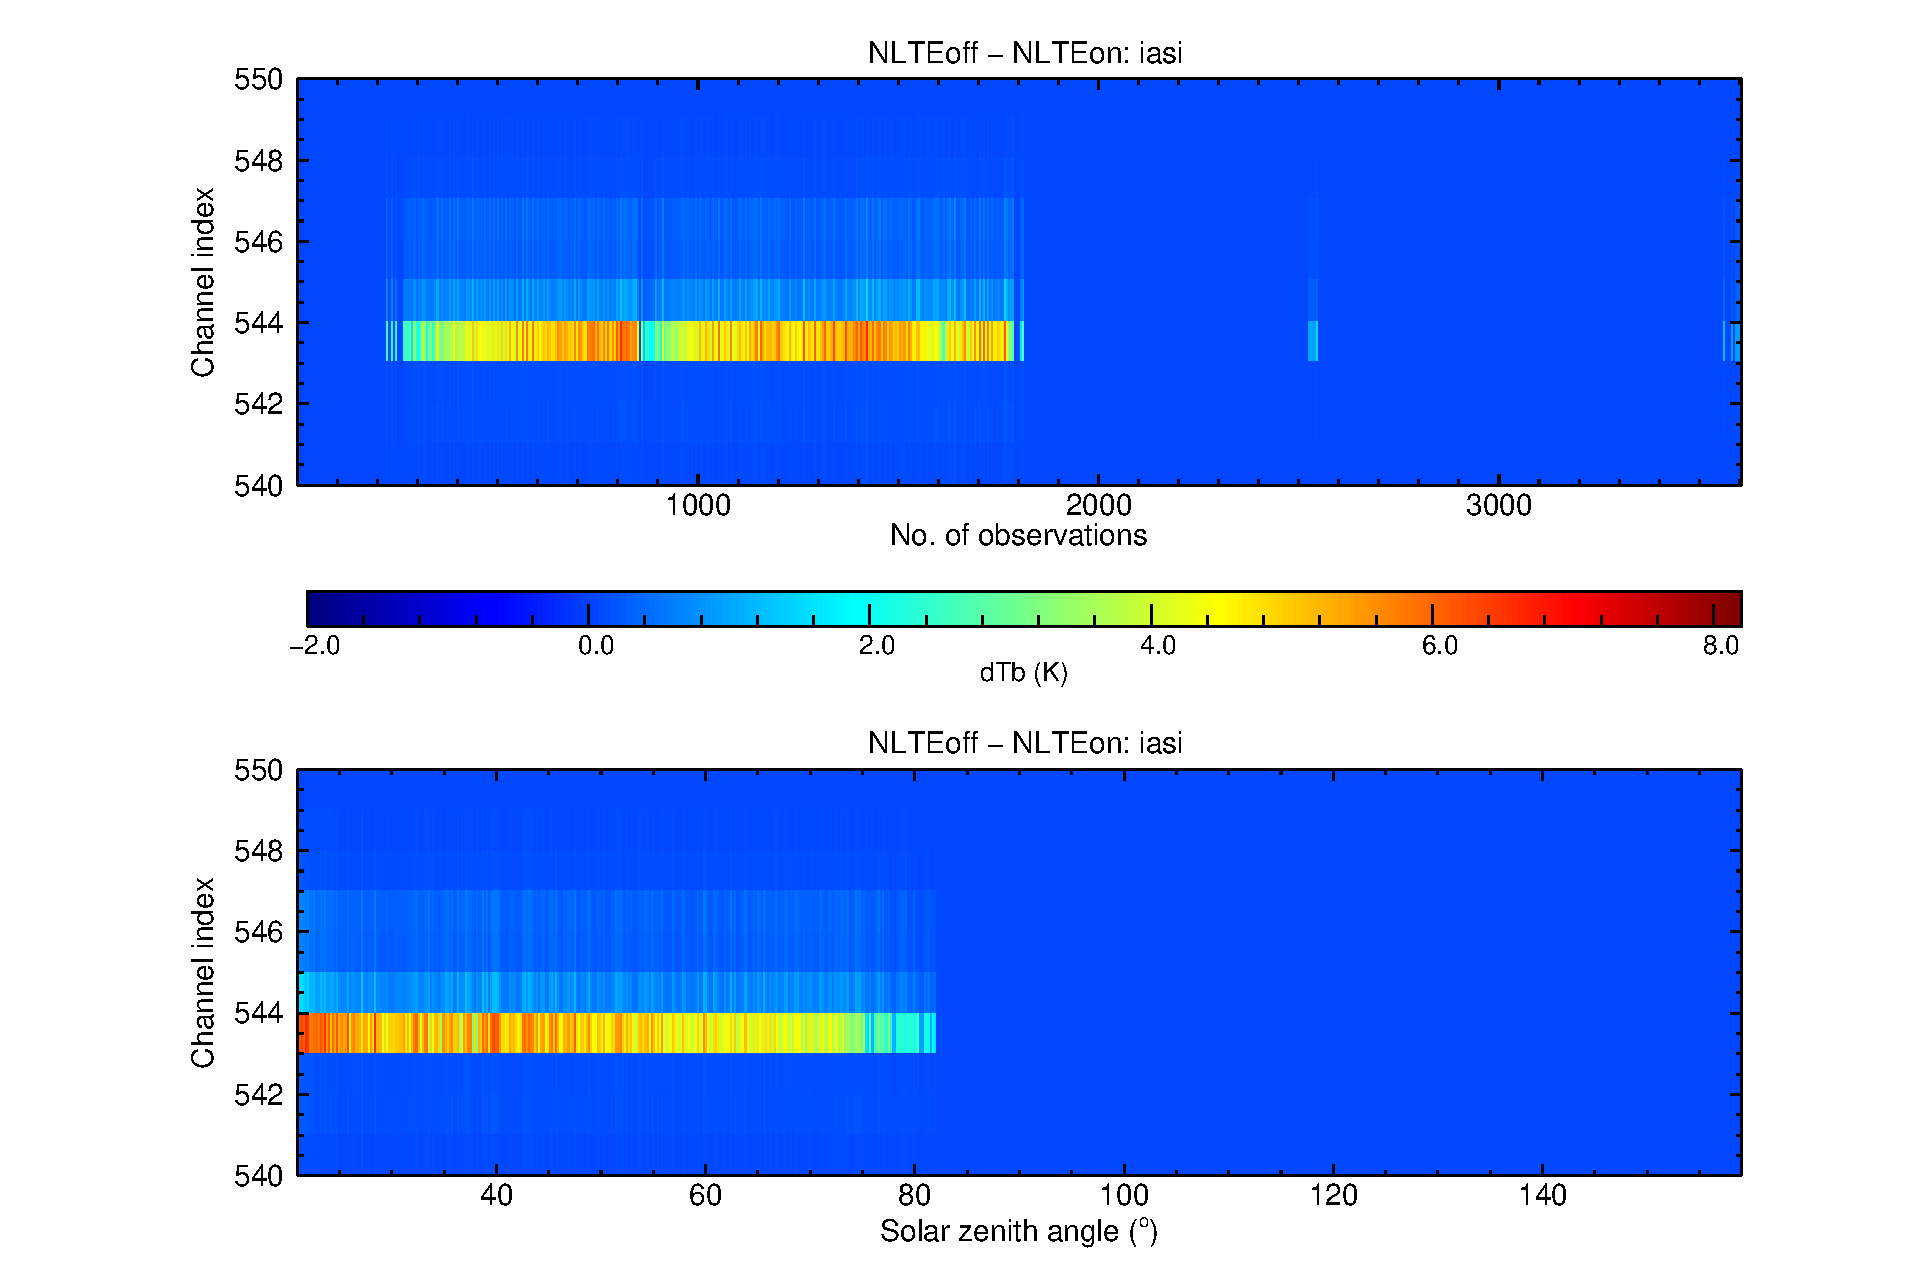
\includegraphics[bb=80 0 840 600,clip,scale=0.6]{graphics/New/NLTE/iasi_metop-a.eps}
  \caption[Effect of NLTE changes in affected MetOp-A IASI channels]{GSI single-cycle run (2012070200) results for NLTE-affected MetOp-A IASI channels. The brightness temperature differences are shown as a function of observation (top panel) as well as solar zenith angle (bottom panel). The channel indices are for the 616 channel subset used in NCEP. The channel indices shown correspond to channels in the frequency range 2236.25-2391.00cm\ensuremath{^\textsf{-1}}.}
  \label{fig:nlte_impact_iasi_metop-a}
\end{figure}


\section*{New Functionality}
%---------------------------
\addcontentsline{toc}{section}{New Functionality}

\begin{description}
\item[Aerosol optical depth functions] Separate functions to compute just the aerosol optical depth have been implemented. The new main level forward, tangent-linear, adjoint, and K-matrix functions are \f{CRTM\_AOD()}, \f{CRTM\_AOD\_TL()}, \f{CRTM\_AOD\_AD()}, and \f{CRTM\_AOD\_K()} respectively. See section \ref{sec:interface-aod} for the function interfaces.

\item[Channel subsetting] To allow users to select which channels of a sensor will be processed, a channel subsetting function has been added. This subsetting operates on the \ChannelInfo structure and is invoked by passing the list of required channel numbers to a new \f{CRTM\_ChannelInfo\_Subset()} function. See section \ref{sec:init_step-channel_subset} for usage examples and section \ref{sec:CRTM_ChannelInfo_Subset_interface} for the function interface.

\item[Number of streams option] For scattering atmospheres the current method to determine the number of streams to be employed in the radiative transfer calculation is based upon the Mie parameter. Generally this methodology yields a higher number of streams than is necessary. A better ``stream selection'' method is under development and is slated for the v2.2 CRTM release. Part of this work led to the implementation of an \f{n\_Streams} option - that is, the user can explicitly state the number of streams they wish to use for scattering calculations and override any value determined internally. The user-define number of streams is set via the options input to the CRTM functions.

\item[Scattering switch option for clouds and aerosols] This implements a user-selectable switch to ``skip'' the scattering computations and only compute the cloud and aerosol absorption component when clouds and aerosols are present. The scattering switch is set via the options input to the CRTM functions.

\item[Aircraft instrument capability] The ability to simulate an aircraft instrument has been implemented in the CRTM. The user indicates that the calculation is for an aircraft instrument by specifying the flight level pressure in the options input to the CRTM functions. Note, however, that no spectral or transmittance coefficients are available for aircraft instruments. If you wish to run the CRTM for a particular aircraft sensor (microwave, infrared or visible) email the CRTM developers at \href{mailto:ncep.list.emc.jcsda_crtm.support@noaa.gov}{ncep.list.emc.jcsda\_crtm.support@noaa.gov}.

\item[Options structure I/O] Previously, the CRTM \Options structure was different from the other user accessible CRTM structures (e.g. \Atmosphere, \Surface, \Geometry, etc) in that there were no means to write and read the structure to/from file. This oversight has been corrected. See section \ref{sec:options_structure} for the function interfaces.

\end{description}


\section*{Interface Changes}
%---------------------------
\addcontentsline{toc}{section}{Interface Changes}
\label{sec:new_interface_changes}

\begin{description}
\item[Surface type specification changes] The specification of surface type in the CRTM surface structure was previously hardwired to use the NPOESS land surface classification scheme (infrared and visible spectral regions only). For users that employed a different land surface classification scheme, in particular those from USGS or IGBP, it meant there was a classification scheme remapping that was required to assign the ``correct'' NPOESS surface type for a particular USGS or IGBP surface type. To avoid the need to do this remapping, the land surface reflectivity data has now been provided in terms of three surface classification schemes: NPOESS (the default), USGS, and IGBP. These are loaded into the CRTM during the initialization stage.

Previously land surface type parameters such as \f{SCRUB} or \f{BROADLEAF\_FOREST} were available to refer to a unique surface type index that was used to reference a look up table of spectral reflectances. Now, however, the list of allowable surface types can be different based on the classification scheme with which the CRTM was initialized, and thus the numeric index for a surface type in the list is no longer unique to that surface type. This means there can no longer be a list of pre-specified parameterized surface types like there was with v2.0.x of the CRTM.

Tables \ref{tab:npoess_surface_type_classifications}, \ref{tab:usgs_surface_type_classifications}, and \ref{tab:igbp_surface_type_classifications} show the surface types, and their index, available for the NPOESS, USGS, and IGBP land surface classification schemes respectively.

\item[Emissivity model initialisation file changes] In the v2.0.x CRTM the only emissivity/reflectivity model data loaded during initialisation was that for the infrared sea surface emissivity model. Now datafiles are explicitly loaded for each spectral type (infrared, microwave, and visible) as well as each main surface type (land, water, snow, and ice). This was done to get set up for planned future changes and updates to the emissivity and reflectivity models for various spectral regions and surface types.

In general you can rely on the default data files loaded. See table \ref{tab:emiscoeff_file_choices} for a list of available data files and their associated optional argument to the CRTM initialisation function.

\end{description}


To migrate from the CRTM v2.0.x initialisation and surface type specification to that implemented in v2.1, see Appendix \ref{chapter:migration_path}, ``\hyperref[chapter:migration_path]{Migration Path from REL-2.0 to REL-2.1}.''


